The appearance of the UI will be described in this chapter.

\section{Design language and UI framework}
Because the application should look decent, some UI guidelines have to be chosen and followed.
These guidelines cover information about colors, shapes and individual components, including their layout.
A set of these guidelines is called design language.
Following design languages are suitable for the Android platform due to the existence of frameworks for this platform, containing themes and components of those languages.

Bootstrap \cite{bootstrap} is a framework for designing web pages, but there also exists a third party library \cite{androidbootstrap} for the Android platform.
Both Microsoft Fluent Design System \cite{fluentui} and Material Design \cite{materialandroid} have their own official libraries available from their representative web pages.

The Bootstrap Android library has not been updated since December 2016 and considering that UI design is always changing and evolving, this library is out of question.
Both Microsoft Fluent Design System and Material Design are being kept up-to-date and are backed by big international companies, which should ensure their stability.
Because our application will be available on the Android platform, which is Google's domain and most Android phones come with several Google applications pre-installed, Android users are already used to Material Design.

That is why Material Design will be used by our application.

\section{Main screens}
Based on the analysis of the user requirements in \autoref{chap:requirementsengineering}, three screens which cover the functionality of displaying execution history, pipeline list and settings have to be designed.

\section{Main navigation}
On the Android platform, there are multiple navigation designs and they will be described in this section.

\subsection{Navigation drawer}
The hamburger icon at the top left and sliding menu from left to right is what the navigation drawer looks like.
This navigation is suitable for five or more top level screens, or some sort of hierarchical menu \cite{navigationdrawer}.

\subsection{Tabs}
Slidable tabs on top of the screen.
% Recommendation for this type of navigation is having at least two screens.\cite{materialandroid}
Users can click on tab names or just slide left or right in order to navigate between the screens.

\subsection{Bottom navigation}
Bottom navigation consists of icons, usually with text, located at the bottom of the screen.

\section{Conclusion about the main navigation}
The navigation drawer will not be used, because our application does not require five or more main screens nor a hierarchical menu.
Also, with the increasing sizes of mobile phones and most people being right-handed, it is hard to reach the hamburger menu with the right thumb.
There will be lists of items displayed on each of the three main screens.
Those items will be swipeable and having swipeable items on top of swipeable navigation would cause confusion.
Material Design states that the recommended number of links in the bottom navigation is three to five \cite{bottomnavigation}.
The bottom navigation satisfies our needs and will be used for the main navigation.
The three main screens, containing the bottom navigation, can be seen in \autoref{fig:xdHistory}, \autoref{fig:xdPipelines} and \autoref{fig:xdSettings}.

\begin{figure}\centering
    \begin{minipage}[b]{0.32\textwidth}
    	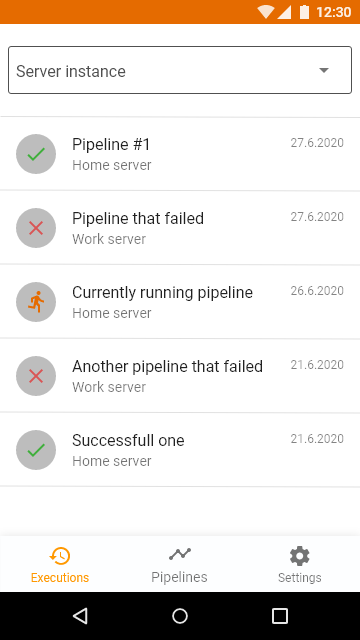
\includegraphics[width=\textwidth]{pics/xd/Bottom Navigation - executions.png}
    	\caption[History]{History screen design}\label{fig:xdHistory}
    \end{minipage}
    \begin{minipage}[b]{0.32\textwidth}
    	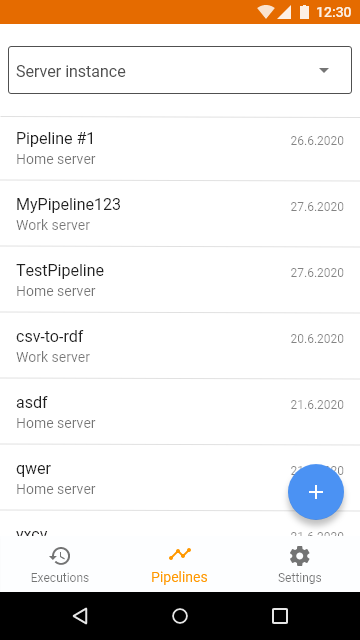
\includegraphics[width=\textwidth]{pics/xd/Bottom Navigation - pipelines.png}
    	\caption[Pipelines]{Pipelines screen design}\label{fig:xdPipelines}
    \end{minipage}
    \begin{minipage}[b]{0.32\textwidth}
    	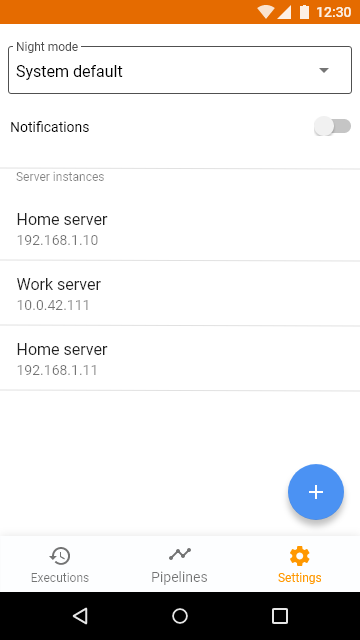
\includegraphics[width=\textwidth]{pics/xd/Bottom Navigation - settings.png}
    	\caption[Settings]{Settings screen design}\label{fig:xdSettings}
    \end{minipage}
\end{figure}

\section{Lists}
Each of the three main screens will display some sort of list.
For the execution screen it is a list of executions, for the pipeline screen it is a list of pipelines and for the settings screen it is a list of server instances.

All of those lists will have one thing in common and that being the swipe gesture.
When users swipe an item to the left or to the right, the item will be deleted.
This can be seen in \autoref{fig:xdDeletePipeline}.
Users will have the ability to undo this operation for a short period of time.
The undo option can be seen in \autoref{fig:xdUndo}.

Tapping on an item from the pipeline screen will open the edit pipeline screen.
Long click on item from execution screen or from pipeline screen will launch the pipeline.

\begin{figure}\centering
    \begin{minipage}[b]{0.32\textwidth}
    	\includegraphics[width=\textwidth]{pics/xd/Bottom Navigation - pipelines – 1.png}
    	\caption[Deleting pipeline]{Deleting pipeline design}\label{fig:xdDeletePipeline}
    \end{minipage}
    \begin{minipage}[b]{0.32\textwidth}
    	\includegraphics[width=\textwidth]{pics/xd/Bottom Navigation - pipelines – 2.png}
    	\caption[Undo option]{Undo option design}\label{fig:xdUndo}
    \end{minipage}
\end{figure}

\section{Edit server instance screen}
While registering a new server instance or editing an already registered one, the application needs the address for communication and some name for labeling and better organising.
Users will be able to add a description of the instance, so that there is no pressure to store every information about the instance in the server name.
There could also be an option to ping the server (F-2.6, \autoref{subsec:ping}) to verify the address and a way to cancel the registration/edit.
Because of this, another screen, just for registering/editing server instances, will be added and can be seen in \autoref{fig:xdEditServerInstance}.

\begin{figure}\centering
    \begin{minipage}[b]{0.32\textwidth}
    	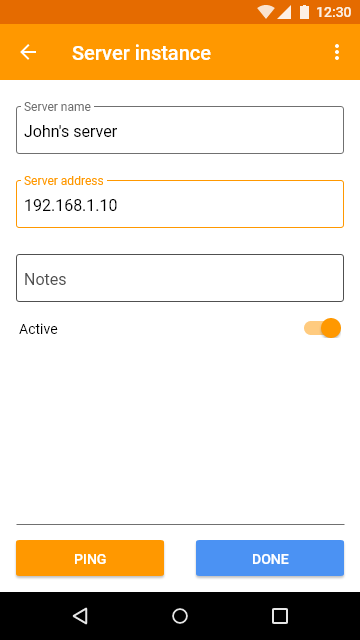
\includegraphics[width=\textwidth]{pics/xd/Edit server instance.png}
    	\caption[Edit server instance]{Edit server instance screen design}\label{fig:xdEditServerInstance}
    \end{minipage}
    \begin{minipage}[b]{0.32\textwidth}
    	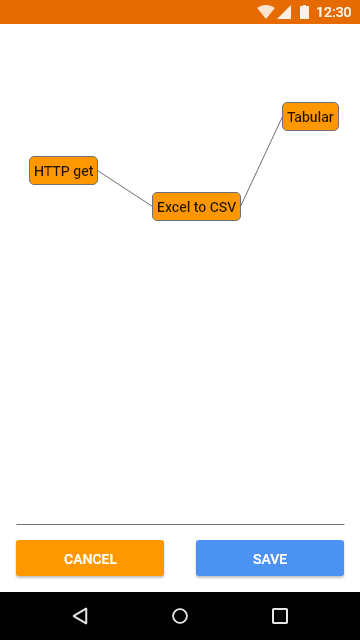
\includegraphics[width=\textwidth]{pics/xd/Pipeline editor.png}
    	\caption[Edit pipeline screen]{Edit pipeline screen design}\label{fig:xdPipelineEditor}
    \end{minipage}
\end{figure}

\section{Edit pipeline screen}
According to the F-4.3 requirement, described in \autoref{subsec:editpipelinescreen}, there has to be a screen for editing pipelines.
This screen will be displaying pipeline components and drawing links between them.
The preliminary design of this screen can be seen in \autoref{fig:xdPipelineEditor}

% \begin{figure}\centering
%     \begin{minipage}[b]{0.32\textwidth}
%     	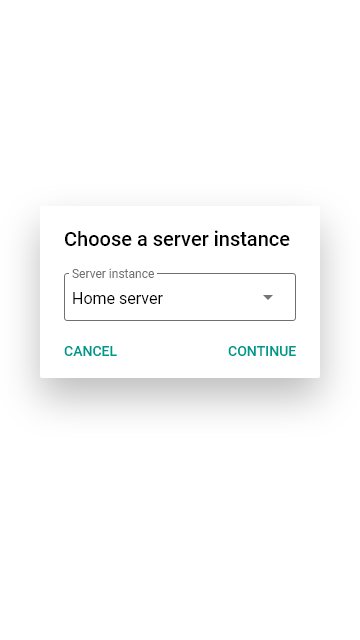
\includegraphics[width=\textwidth]{pics/xd/Create new pipeline.png}
%     	\caption[Create new pipeline dialog]{Create new pipeline dialog design}\label{fig:xdCreateNewPipelineDialog}
%     \end{minipage}
%     \begin{minipage}[b]{0.32\textwidth}
%     	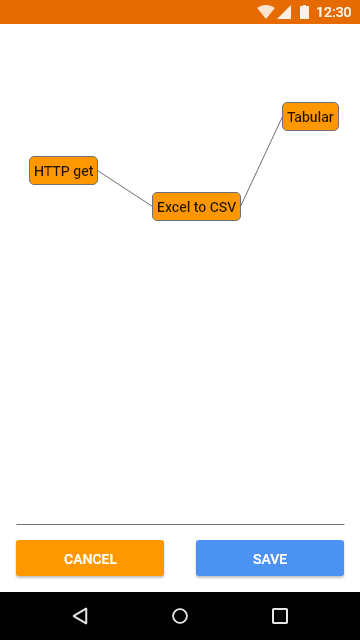
\includegraphics[width=\textwidth]{pics/xd/Pipeline editor.png}
%     	\caption[Edit pipeline screen]{Edit pipeline screen design}\label{fig:xdPipelineEditor}
%     \end{minipage}
% \end{figure}

\section{Edit component screen}
This screen has to be created, because each pipeline's component has its own settings.
In \autoref{fig:xdEditComponent1} and \autoref{fig:xdEditComponent2} is the preliminary design of this screen.

\begin{figure}\centering
    \begin{minipage}[b]{0.32\textwidth}
    	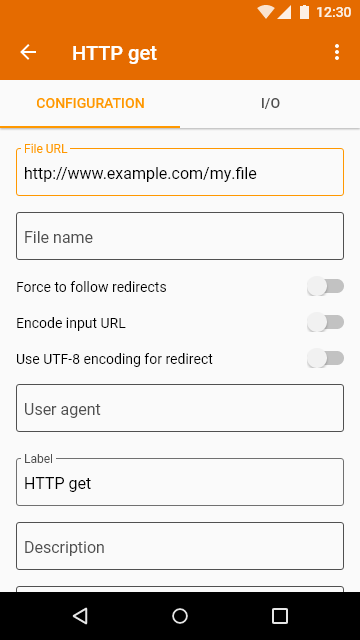
\includegraphics[width=\textwidth]{pics/xd/Edit component - configuration.png}
    	\caption[Edit component screen 1]{Edit component screen 1 design}\label{fig:xdEditComponent1}
    \end{minipage}
    \begin{minipage}[b]{0.32\textwidth}
    	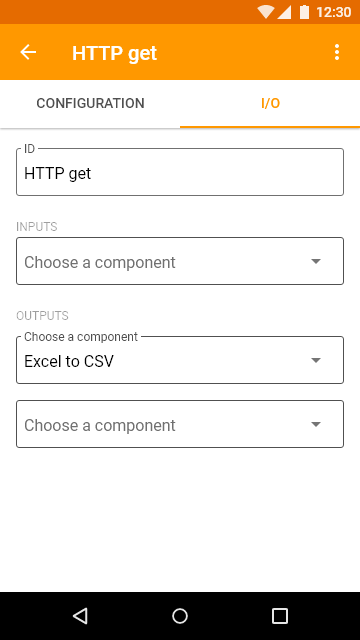
\includegraphics[width=\textwidth]{pics/xd/Edit component - io.png}
    	\caption[Edit component screen 2]{Edit component screen 2 design}\label{fig:xdEditComponent2}
    \end{minipage}
\end{figure}

\section{Notifications}
According to the F-3.1 requirement, described in \autoref{subsec:notifications}, notifications need to be implemented.
The preview of notifications can be seen in \autoref{fig:xdNotifications}.

\begin{figure}\centering
    \begin{minipage}[b]{0.7\textwidth}
    	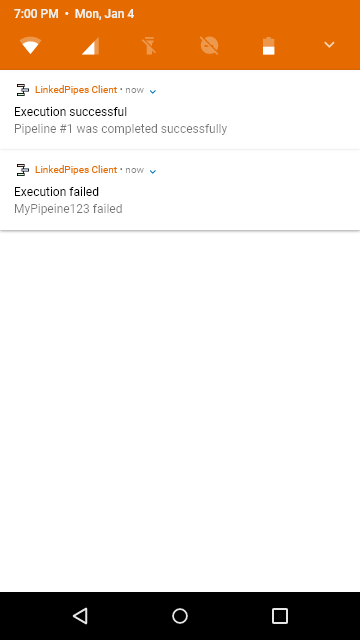
\includegraphics[width=\textwidth]{pics/xd/Notifications.png}
    	\caption[Notifications]{Notification design}\label{fig:xdNotifications}
    \end{minipage}
\end{figure}